\section{Rectilinear movement dynamics with $r_{flywheel}$ fixed}

In order to study the dynamics of the robot we will use Lagrange mechanics.
To reduce the number of variables we wil study the case of rectilinear
movement by imposing that both wheels turn at the same speed. We will also set
the radius of the free weight to $r_{flywheel}$.

The generalized coordinates ($q$) will be:
\begin{enumerate}
	\item $\phi_{ground-wheel}$: rotation of the wheel respect the ground.
	\item $\phi_{wheel-platform}$: rotation of the platform respect the wheel.
	\item $\phi_{platform-flywheel}$: rotation of the flywheel respect the platform.
\end{enumerate}

We will use two auxiliary variables:
\begin{enumerate}
	\item $\phi_{ground-platform}=\phi_{ground-wheel}+\phi_{wheel-platform}$: rotation of the platform respect the ground.
	\item $\phi_{ground-flywheel}=\phi_{ground-platform}+\phi_{platform-flywheel}$: rotation of the flywheel respect the ground.
\end{enumerate}

The total potential energy:
\begin{equation}
	V = m_{cylinder}\cdot (r_{flywheel}-r_{flywheel-max}) \cdot cos(\phi_{ground-flywheel}) \cdot g
\end{equation}


The total kinetic energy:
\begin{equation}
	T = \frac{1}{2}\cdot[\dot{\phi}_{ground-wheel}^2\cdot I_{wheel}
		+ \dot{\phi}_{ground-platform}^2 \cdot I_{platform}
		+ \dot{\phi}_{ground-flywheel}^2\cdot I_{flywheel}
		+ \dot{\phi}_{ground-wheel}^2\cdot r_{wheel}^2\cdot m_{total}]
\end{equation}

The Lagrangian is defined as:
\begin{equation}
	L=T-V
\end{equation}

Lagrange's equation is:
\begin{equation}
	\frac{d}{dt}(\frac{\partial L}{\partial \dot{q}_j})=
	\frac{\partial L}{\partial q_j}	+ F_{j}
\end{equation}

So in our case:
\begin{equation}
	\frac{\partial L}{\partial \dot{\phi}_{ground-wheel}}=
	\dot{\phi}_{ground-wheel} \cdot I_{wheel}
	+ \dot{\phi}_{ground-platform} \cdot I_{platform}
	+ \dot{\phi}_{ground-flywheel}\cdot I_{flywheel}
	+ \dot{\phi}_{ground-wheel}\cdot r_{wheel}^2\cdot m_{total}
\end{equation}

\begin{equation}
	\frac{\partial L}{\partial \dot{\phi}_{wheel-platform}}=
	\dot{\phi}_{ground-platform} \cdot I_{platform}
	+ \dot{\phi}_{ground-flywheel}\cdot I_{flywheel}
\end{equation}

\begin{equation}
	\frac{\partial L}{\partial \dot{\phi}_{platform-flywheel}}=
	\dot{\phi}_{ground-flywheel}\cdot I_{flywheel}
\end{equation}

We define M as the following matrix:
\begin{equation}
	\begin{pmatrix}
		I_{wheel} + I_{platform} + I_{flywheel} + r_{wheel}^2 \cdot m_{total} &
		I_{platform} + I_{flywheel}                                           &
		I_{flywheel}                                                            \\
		I_{platform} + I_{flywheel}                                           &
		I_{platform} + I_{flywheel}                                           &
		I_{flywheel}                                                            \\
		I_{flywheel}                                                          &
		I_{flywheel}                                                          &
		I_{flywheel}                                                            \\
	\end{pmatrix}
\end{equation}

In matrix form and with our generalized coordinates:
\begin{equation}
	\frac{\partial L}{\partial \dot{q}} =
	M \cdot \dot{q}
\end{equation}

\begin{equation}
	\frac{d}{dt}(\frac{\partial L}{\partial \dot{q}}) = 	M \cdot \ddot{q}
\end{equation}

Let a be a constant:
\begin{equation}
	a = m_{cylinder}\cdot (r_{flywheel}-r_{flywheel-max}) \cdot g
\end{equation}

\begin{equation}
	\frac{\partial L}{\partial q} = a \cdot sin(\phi_{ground-flywheel}) \cdot
	\begin{pmatrix}
		1 \\ 1 \\ 1
	\end{pmatrix}
\end{equation}

So using Lagrange's equation we get:
\begin{equation}
	\boxed{
		M \cdot \ddot{q} = a \cdot sin(\phi_{ground-flywheel}) \cdot
		\begin{pmatrix}
			1 \\ 1 \\ 1
		\end{pmatrix} + F
	}
\end{equation}


\subsection{Simulations}
In this subsection we study different policies for the external forces
($F$) applied to the robot in rectilinear movement case.

The robot has 2 actuators, the motors between the wheel and the platform
and the motor between the flywheel and the platform.
All motors in the systems  have a limited torque related with the
speed as you may see in Figure \ref{fig: Motor torque}.

\begin{equation}
	\boxed{
		F =
		\begin{pmatrix}
			0 \\ \tau_{wheel-platform} \\ \tau_{platform-flywheel}
		\end{pmatrix}
	}
\end{equation}

In order to compare the different policies all of them have the same target.
The robot must travel 30 radiants (3 meters) and stop at the end. All the parameters from 
the simulation are set equal to the values found in section \ref{sec: parameters results}.
Keep in mind that the wheel radius is 10 cm.

Here you can see a table that summarize the results:
\begin{center}
	\begin{tabular}{ |c|c|c|c|c|c|c| } 
	 \hline
	 \textbf{Experiment} & \textbf{Total time(s)} & \textbf{Time to max speed(s)} 
	 & \textbf{Max speed(rad/s)} & \textbf{Time to brake(s)}\\
	 \hline
	 \textbf{Controlling inclination} \\
	 \hline
	 Flywheel & 12,45 & 0,7 & 2,45 & 0,15\\
	 \hline
	 Pendulum & 5,59 & 2,69 & 10,36 & 2,90\\
	 \hline
	 Waitress & 8,24 & 4,12 & 5,49 & 4,12\\
	 \hline
	 \textbf{Free inclination} \\
	 \hline
	 Double flywheel & 3,9 & 1 & 8,51 & 0.27\\
	 \hline
	 Compose mechanism & 3,82 & 2,3 & 10,2 & 2,04\\
	 \hline
	\end{tabular}
\end{center}

\subsubsection{Controlling the platform inclination}
In the first two experiments we want to keep the platform in an horizontal position.
That's the reason why we force the $ \tau_{wheel-platform}$ equal to
$\tau_{platform-flywheel}$ in the experiments flywheel and pendulum.

\begin{enumerate}
	\item Flywheel
	
		The movable weight is fixed at $r_{max}$. In this experiment we consign the platform-flywheel motor to 
		output the maximum possible torque. Then the platform-wheels motors deliver
		the same torque. The platform-flywheel motor reaches in less than one second
		the maximum speed. This then limits the wheel-platform speed because no
		more torque can by applied one that point is reached.
	      \begin{figure}[H]
		      \centering
		      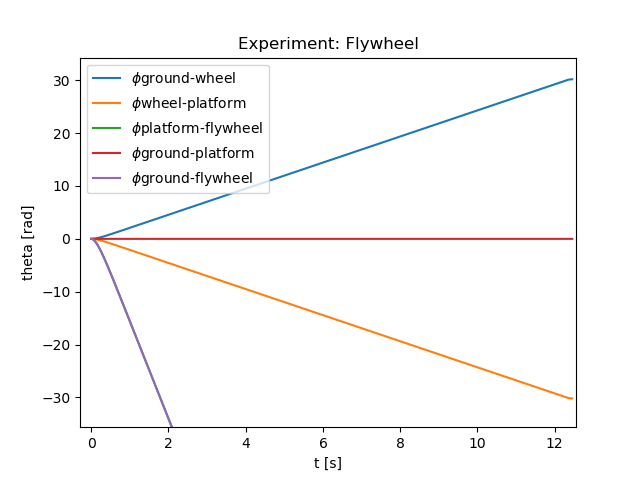
\includegraphics[width=10cm]{img/lagrange_5/flywheel_q.png}
		      \caption{Plot of the angles for the flywheel experiment.}
		      \label{fig:Simulation flywheel q}
	      \end{figure}


	      \begin{figure}[H]
		      \centering
		      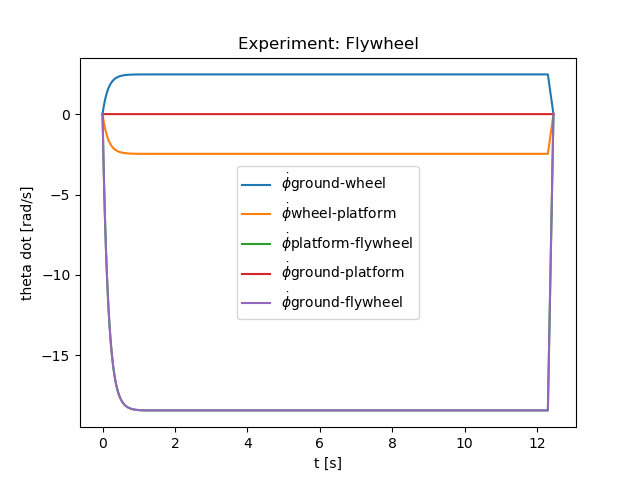
\includegraphics[width=10cm]{img/lagrange_5/flywheel_q_dot.png}
		      \caption{Plot of the angular velocities for the flywheel experiment.}
		      \label{fig:Simulation flywheel q dot}
	      \end{figure}
	\item Pendulum
	
		The movable weight is fixed at $r_{min}$. In this experiment we consign the platform-flywheel motor to 
		get to 90º with a PID controller. Then the platform-wheels motors deliver
		the same torque. The robot does not accelerate as fast as in the flywheel
		experiment but reaches a higher speed that allows it to travel the distance
		in less time. Note that the robot could have kept accelerating but had to
		brake before reaching the maximum speed. 
	      \
	      \begin{figure}[H]
		      \centering
		      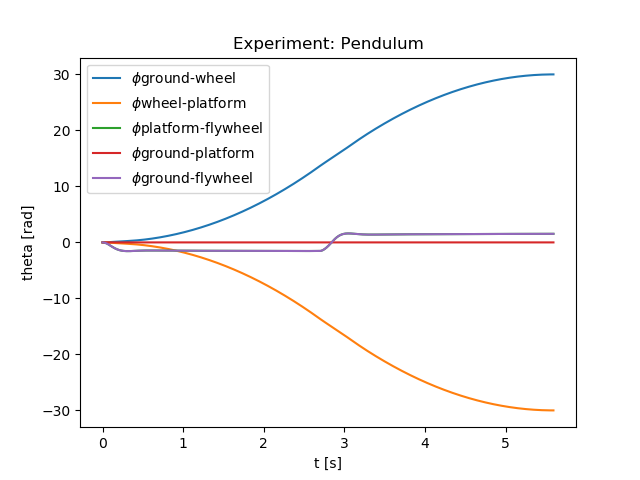
\includegraphics[width=10cm]{img/lagrange_5/pendulum_q.png}
		      \caption{Plot of the angles for the pendulum experiment.}
		      \label{fig:Simulation pendulum q}
	      \end{figure}


	      \begin{figure}[H]
		      \centering
		      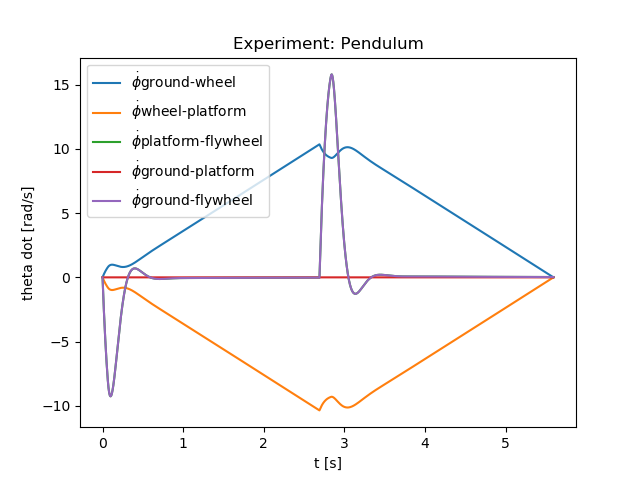
\includegraphics[width=10cm]{img/lagrange_5/pendulum_q_dot.png}
		      \caption{Plot of the angular velocities for the pendulum experiment.}
		      \label{fig:Simulation pendulum q dot}
	      \end{figure}
	\item Waitress
	
	The movable weight is fixed at $r_{min}$. This experiment is different that the previous two and it's aim is to illustrate
		  how the robot could follow and inclination consign. The experiment is designed
		  the following way. A consign torque is given to the wheel-platform and the
		  flywheel-motor PID has an inclination consign too. The inclination consign is such
		  that the sum of accelerations received from and object in the platform is perpendicular
		  to the platform. 



	      \begin{figure}[H]
		      \centering
		      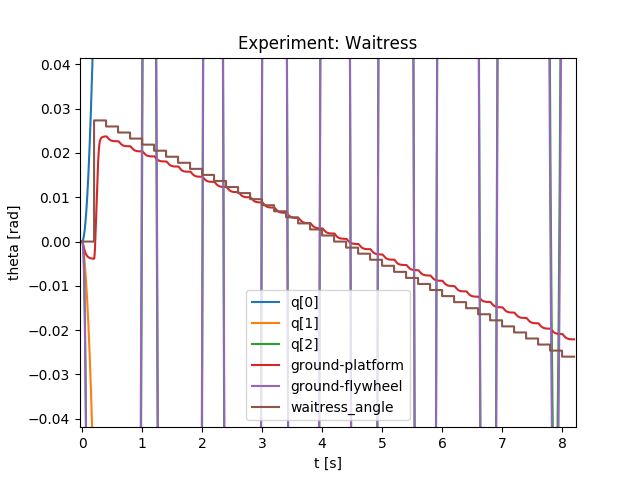
\includegraphics[width=10cm]{img/lagrange_5/waitress_q_zoom.png}
		      \caption{Plot of the angles for the waitress experiment.}
		      \label{fig:Simulation pendulum q}
	      \end{figure}


	      \begin{figure}[H]
		      \centering
		      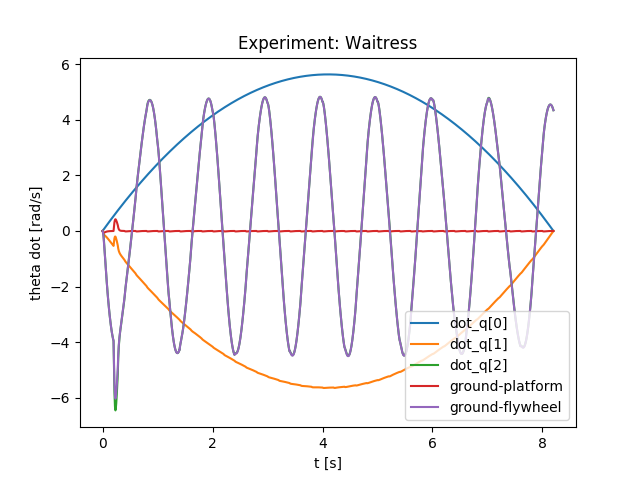
\includegraphics[width=10cm]{img/lagrange_5/waitress_q_dot.png}
		      \caption{Plot of the angular velocities for the waitress experiment.}
		      \label{fig:Simulation pendulum q dot}
	      \end{figure}

\end{enumerate}
\subsubsection{Letting the platform turn}
In this experiment we take advantage of the fact that the platform may not be needed
to stay horizontal in some displacement. The robot uses the platform as an
additional flywheel to help the robot accelerate and brake.
\begin{enumerate}
	\item Double Flywheel
	
	The movable weight is fixed at $r_{max}$. In this experiment we add the flywheel turn over the platform turn to 
		create more torque to accelerate our wheels. We always do the maximum possible torque with all the motors.
	      \begin{figure}[H]
		      \centering
		      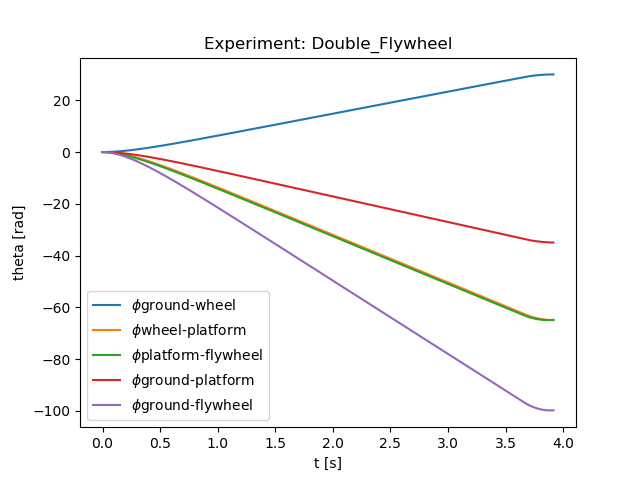
\includegraphics[width=10cm]{img/lagrange_5/double_q.png}
		      \caption{Plot of the angles for the double flywheel experiment.}
		      \label{fig:Simulation double q}
	      \end{figure}


	      \begin{figure}[H]
		      \centering
		      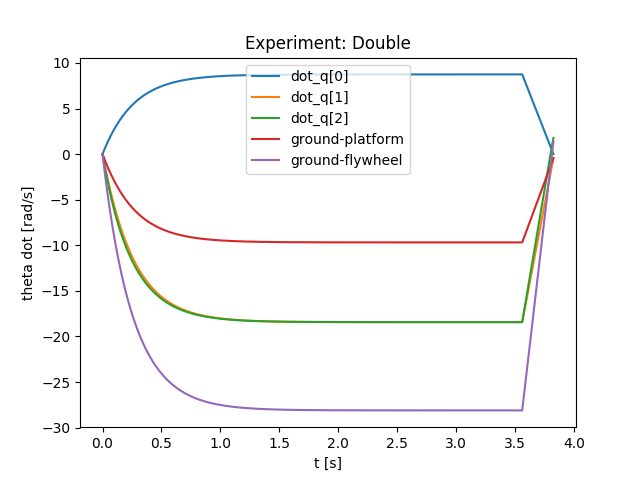
\includegraphics[width=10cm]{img/lagrange_5/double_q_dot.png}
		      \caption{Plot of the angular velocities for the double flywheel experiment.}
		      \label{fig:Simulation double q dot}
	      \end{figure}
	\item Compose
		  
	The movable weight is fixed at $r_{min}$. In this experiment we add the pendulum effect to the flywheel effect produced
		  by the flywheel. We do so with a PID controller for the angle ground-flywheel and making the maximum possible torque
		  with the platform-wheel motors. 
	      \begin{figure}[H]
		      \centering
		      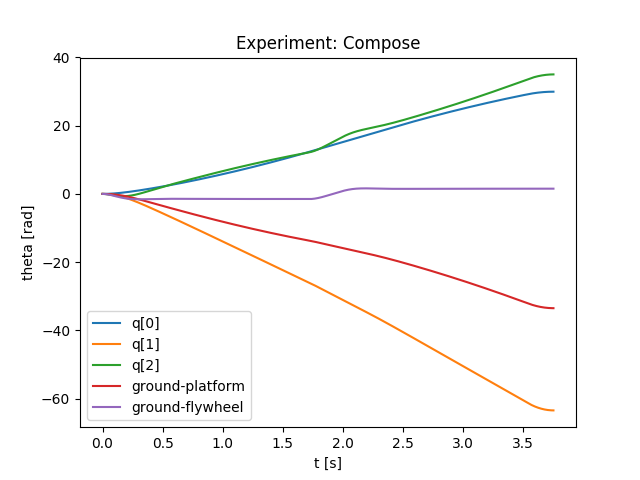
\includegraphics[width=10cm]{img/lagrange_5/compose_q.png}
		      \caption{Plot of the angles for the compose experiment.}
		      \label{fig:Simulation compose q}
	      \end{figure}


	      \begin{figure}[H]
		      \centering
		      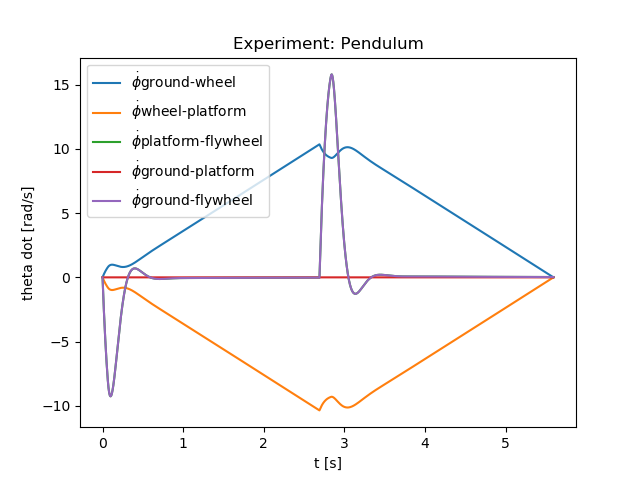
\includegraphics[width=10cm]{img/lagrange_5/pendulum_q_dot.png}
		      \caption{Plot of the angular velocities for the pendulum experiment.}
		      \label{fig:Simulation compose q dot}
	      \end{figure}
\end{enumerate}



\subsection{Rectilinear movement with $r_{flywheel}$ free}

The generalized coordinates ($q$) will be:
\begin{enumerate}
	\item $\phi_{ground-wheel}$: rotation of the wheel respect the ground.
	\item $\phi_{wheel-platform}$: rotation of the platform respect the wheel.
	\item $\phi_{platform-flywheel}$: rotation of the flywheel respect the platform.
	\item $r$: distance from the center of the flywheel of the free cylinder.

\end{enumerate}

We will use two auxiliary variables:
\begin{enumerate}
	\item $\phi_{ground-platform}=\phi_{ground-wheel}+\phi_{wheel-platform}$: rotation of the platform respect the ground.
	\item $\phi_{ground-flywheel}=\phi_{ground-platform}+\phi_{platform-flywheel}$: rotation of the flywheel respect the ground.
\end{enumerate}

The total potential energy:
\begin{equation}
	V = m_{cylinder}\cdot (r-r_{flywheel-max}) \cdot cos(\phi_{ground-flywheel}) \cdot g
\end{equation}


The total kinetic energy:
\begin{multline}
	T = \frac{1}{2}\cdot[\dot{\phi}_{ground-wheel}^2\cdot I_{wheel}
		+ \dot{\phi}_{ground-platform}^2 \cdot I_{platform}
		+ \dot{\phi}_{ground-flywheel}^2\cdot I_{flywheel}(r)\\
		+ \dot{\phi}_{ground-wheel}^2\cdot r_{wheel}^2\cdot m_{total}
		+ \dot{r}^2\cdot m_{cylinder}]
\end{multline}

The Lagrangian is defined as:
\begin{equation}
	L=T-V
\end{equation}

Lagrange's equation is:
\begin{equation}
	\frac{d}{dt}(\frac{\partial L}{\partial \dot{q}_j})=
	\frac{\partial L}{\partial q_j}	+ F_{j}
\end{equation}

So in our case:
\begin{multline}
	\frac{\partial L}{\partial \dot{\phi}_{ground-wheel}}=
	\dot{\phi}_{ground-wheel} \cdot I_{wheel}
	+ \dot{\phi}_{ground-platform} \cdot I_{platform}\\
	+ \dot{\phi}_{ground-flywheel}\cdot I_{flywheel}(r)
	+ \dot{\phi}_{ground-wheel}\cdot r_{wheel}^2\cdot m_{total}
\end{multline}

\begin{equation}
	\frac{\partial L}{\partial \dot{\phi}_{wheel-platform}}=
	\dot{\phi}_{ground-platform} \cdot I_{platform}
	+ \dot{\phi}_{ground-flywheel}\cdot I_{flywheel}(r)
\end{equation}

\begin{equation}
	\frac{\partial L}{\partial \dot{\phi}_{platform-flywheel}}=
	\dot{\phi}_{ground-flywheel}\cdot I_{flywheel}(r)
\end{equation}

\begin{equation}
	\frac{\partial L}{\partial \dot{r}}=
	\dot{r}\cdot m_{cylinder}
\end{equation}

We define M as the following matrix:
\begin{equation}
	\begin{pmatrix}
		I_{wheel} + I_{platform} + I_{flywheel}(r) + r_{wheel}^2 \cdot m_{total} &
		I_{platform} + I_{flywheel}(r)                                           &
		I_{flywheel}(r)                                                          &
		0                                                                          \\
		I_{platform} + I_{flywheel}(r)                                           &
		I_{platform} + I_{flywheel}(r)                                           &
		I_{flywheel}(r)                                                          &
		0                                                                          \\
		I_{flywheel}(r)                                                          &
		I_{flywheel}(r)                                                          &
		I_{flywheel}(r)                                                          &
		0                                                                          \\
		0                                                                        &
		0                                                                        &
		0                                                                        &
		m_{cylinder}                                                               \\
	\end{pmatrix}
\end{equation}

In matrix form and with our generalized coordinates:
\begin{equation}
	\frac{\partial L}{\partial \dot{q}} =
	M \cdot \dot{q}
\end{equation}

\begin{equation}
	\frac{d}{dt}(\frac{\partial L}{\partial \dot{q}}) =
	M \cdot \ddot{q} + \dot{M} \cdot \dot{q}
\end{equation}

Let's recall the definition of $I_{flywheel}(r)$
\begin{equation}
	I_{flywheel}(r)= m_{cylinder} \cdot r^2 + C
\end{equation}


Compute the derivative
\begin{equation}
	\dot{I}_{flywheel}(r)= 2 \cdot m_{cylinder} \cdot r \cdot \dot{r}
\end{equation}

We compute $\dot{M}$ as the following matrix:
\begin{equation}
	\dot{M}=
	\dot{I}_{flywheel}(r) \cdot
	\begin{pmatrix}
		1 &
		1 &
		1 &
		0   \\
		1 &
		1 &
		1 &
		0   \\
		1 &
		1 &
		1 &
		0   \\
		0 &
		0 &
		0 &
		0   \\
	\end{pmatrix}
\end{equation}

Let $a$ be::
\begin{equation}
	\frac{\partial L}{\partial q_{1..3}} = a = m_{cylinder}\cdot (r-r_{flywheel-max}) \cdot g \cdot sin(\phi_{ground-flywheel})
\end{equation}

Let $b$ be:
\begin{equation}
	\frac{\partial L}{\partial r} = b = \cdot m_{cylinder} \cdot r  \cdot \dot{\phi}_{ground-flywheel}^2  - m_{cylinder}\cdot g \cdot cos(\phi_{ground-flywheel})
\end{equation}

\begin{equation}
	\frac{\partial L}{\partial q} = \begin{pmatrix}
		a \\ a \\ a \\ b
	\end{pmatrix}
\end{equation}

So using Lagrange's equation we get:
\begin{equation}
	\boxed{
		M \cdot \ddot{q} + \dot{M} \cdot \dot{q}=
		\begin{pmatrix}
			a \\ a \\ a \\ b
		\end{pmatrix}
		+ F
	}
\end{equation}
